\documentclass[a4paper,twoside]{article}

\usepackage{epsfig}
% \usepackage{calc}
\usepackage{amssymb}
\usepackage{amstext}
\usepackage{amsmath}
\usepackage{amsthm}
\usepackage{multicol}
\usepackage{pslatex}
\usepackage{apalike}
\usepackage{SCITEPRESS}
\usepackage[small]{caption}

\usepackage{url}
\usepackage{subfig}
\usepackage{graphicx}
\usepackage{epstopdf}
\usepackage{flushend}
\usepackage{listings}
\usepackage{color}
\usepackage{multicol}
\usepackage{amsmath}

\usepackage{floatrow}
\DeclareFloatFont{tiny}{\tiny}% "scriptsize" is defined by floatrow, "tiny" not
\floatsetup[table]{font=tiny}

\newtheorem{definition}{Definition}

% correct bad hyphenation here
\hyphenation{op-tical net-works semi-conduc-tor}



\definecolor{dkgreen}{rgb}{0,0.6,0}
\definecolor{gray}{rgb}{0.5,0.5,0.5}
\definecolor{mauve}{rgb}{0.58,0,0.82}

\lstset{
  language=Java,
  aboveskip=3mm,
  belowskip=3mm,
  showstringspaces=false,
  columns=flexible,
  basicstyle={\footnotesize\ttfamily},
  numbers=none,
  numberstyle=\tiny\color{gray},
  keywordstyle=\color{blue},
  commentstyle=\color{dkgreen},
  stringstyle=\color{mauve},
  breaklines=true,
  breakatwhitespace=true
  tabsize=3
}

\lstset{breaklines=true}

\begin{document}

\title{Framework for Collection of Electrophysiology Data}

\author{\authorname{XXX\sup{1}, XXX\sup{1}, XXX\sup{1}, XXX\sup{1}, XXX\sup{2,3,4}, XXX\sup{4}, XXX\sup{4}}
\affiliation{\sup{1}XXX, XXX, XXX, XXX, XXX, XXX}
\affiliation{\sup{2}XXX, XXX, XXX, XXX, XXX, XXX}
\affiliation{\sup{3}XXX, XXX, XXX, XXX, XXX, XXX}
\affiliation{\sup{4}XXX, XXX, XXX, XXX, XXX, XXX}
\email{XXX, XXX, XXX, XXX, XXX, XXX}
}

\keywords{electrophysiology, mobile app, odML, EEGBase, experimental metadata}

\abstract{Experiments in electrophysiology produce a lot of unstructured metadata collected in electrophysiology databases. The data are usually accessed through a web interface implemented on the top of data model respecting given data format. A lot of experiments are conducted outside the laboratory where access to these databases is not always available. The usage of mobile devices such as tablets or smart phones seems to be a practical solution, but users would welcome the same structured user interface such as they know from a common computer. When user interfaces of electrophysiology databases are tailored to a unique data structure, they cannot be easily reused on a mobile device. As a solution, a mapping of a general data structure to a graphical template is proposed. This mapping is implemented in a framework that generates a template representing the database structure. The parsing process is driven by supplemented annotations added to the code. Next, an Android tool visualizing a graphical layout generated from the template is developed. A use case study is presented on a database of EEG/ERP experiments.}

\onecolumn \maketitle \normalsize \vfill

\section{Introduction}\label{Introduction}

Large collections of data sets are obtained during electrophysiological experiments. With increasing number of experiments a crucial task is to provide metadata descriptions. These metadata usually include experimental constraints and scenarios, and information about tested subject. Raw data without descriptive metadata are meaningless. At present, due to the penetration of computers into medicine collections of electrophysiology, metadata are moved from paper forms to specialized electrophysiological databases. These databases are accessed via desktop or web based user interfaces using common computers. However, there are common situations when a classic computer is not available. These situations occur in environments such as hospitals or prisons where a wireless connection is usually unavailable. In addition, a lot of experiments are conducted outside laboratories using portable measuring devices. In this case data are obtained offline and then must be backward synchronized with data stored in an electrophysiological database. Electrophysiological databases are based on specific data models. User interfaces implemented on top of these models are non-transferable to other data models. Development of various user interfaces is time consuming, and they are difficult to maintain, consequently it reduces usability. As a solution we present an annotation based framework that aim is to generate a template for client applications. This template contains description of metadata structure of an electrophysiological database. A graphical layout for a specific device is then generated according to the obtained template.  As a first pilot system we have implemented an Android based system that generates a template for mobile devices such as tablets or cell-phones. These devices are connected to the electrophysiological database through the framework API.

The structure of the paper is following. First, we briefly introduce existing electrophysiological databases and mobile-based approaches. Then, we describe a proposed mapping that maps the data model of a database to a template expressed in a transport format. Next, we introduce an implementation the mapping in the framework. The rest of the paper describes validation of the presented approach as a part of a use-case study in which integration of the framework in EEGBase (XXX - ommited for review process) is demonstrated.

\section{State of the Art}

Research in the electrophysiology domain faces a lack of tools and infrastructure for collecting and processing experimental data. There are several initiatives implementing and providing tools for data processing, electrophysiological databases or hardware devices. We provide a brief overview of these members of the international neuroinformatics community, most of which are involved in the activities coordinated by the International Neuroinformatics Coordinating Facility (INCF)\footnote{http://www.incf.org/}:

\begin{itemize}

\item	CRCNS \cite{CRCNS} provides marketplace and discussion forum for sharing tools and data in neuroscience.
\item	Helmholtz \cite{10.3389/conf.fninf.2013.09.00025} is a framework for creating neuroscience databases that are customized to the needs of individual neurophysiology labs.
\item	Carmen \cite{fgibson:Watson2007} is a virtual laboratory that enables a storage of experimental data, experimental protocols, or analysis code. It designs workflows from the stored code and run them remotely.
\item	INCF Dataspace \cite{dataspace} enables interested research groups to connect to a distributed data file system based on iRods\footnote{http://irods.org/}.
\item	G-Node\footnote{http://www.g-node.org/} provides tools for data access, data management and data sharing, including a data sharing platform (XXX - ommited for review process) based on common data models for electrophysiological data and metadata (XXX - ommited for review process)(XXX - ommited for review process). To structure metadata, G-Node has developed odML, an XML schema for the creation of complex metadata structure in computer-readable format (XXX - ommited for review process). The odML data model is used as standard representation within the G-Node infrastructure. An odML mobile editor (XXX - ommited for review process) is currently being developed as a standalone app for Android and iOS platform. This mobile application enables users to create odML structure natively on the app using a Graphical User Interface and to acquire on the fly experimental metadata. These metadata can be processed or shared. In addition, reusable templates can be designed and stored inside the device and filled in later.
\item	EEGBase (XXX - ommited for review process) is a database of well-described EEG/ERP experimental data sets that enables users to upload, download and manage EEG/ERP experiments. A mobile EEGBase client(XXX - ommited for review process) enables users to collect data from EEG/ERP experiments and provides an online synchronization with EEGBase.



\end{itemize}

The first version of the EEGBase database was accessible via a web based user interfaces that allows acquiring, managing and sharing the experimental metadata from a desktop computer. However, it is not always possible to access the web interface in the course of an experiment. We therefore extended the framework to support the use of mobile devices for acquiring experimental metadata (XXX - ommited for review process). Our first version was limited to the metadata model predefined in the database. Any modification of the metadata model would require a complete update of the User Interface for the mobile client.
As creating and maintaining new user-interfaces is time-consuming and requires extensive development resources, the challenge is to elaborate a solution to optimize the further development of this platform. We are proposing here a unique system that allows the automatic creation of specific graphical layouts for various platforms, including mobile devices, web applications, etc. To address this challenge, we transformed the EEGBase framework to use object annotations (XXX - ommited for review process) for creating internal templates out of the database and convert it into odML. The odML structure is then transmitted to the mobile device, which can generate automatically a graphical layout for rendering the metadata document.
The transformation described here marks a first step towards interoperability of the EEGBase portal with the G-Node portal and the integration of our work to propose a unique mobile platform.

\section{Proposed Framework}\label{Framework}

\subsection{System Restrictions and Requirements}

According to the considerations mentioned in Section \ref{Introduction} we decided to design and implement a tool that facilitates collection of metadata from experiments by a unified interface customizable to the data structure. In order to ensure an immediate usage, the user interface must be easy to generate. In addition, the synchronization of collected data with the electrophysiology database is crucial in the perspective of their sharing and management.

These design goals imply several requirements that the system must fulfill. It must be inherently client-server oriented. The server end must provide a well-known API to be integrated with most common electrophysiology databases. Moreover, server and client must communicate using a unified data format for easy migration across different platforms and to be understandable by various clients.

The client end parses the exported data structure and generates a graphical layout. Once the layout is generated, the user can customize it. When the user has the layout prepared, the client is able to download data from the server or push data stored locally. When the client works offline, the data must be stored in an embedded database and synchronized immediately when the client gets back online.



The idea initially presented in (XXX - ommited for review process) described a client-server system. The server is able to annotate the database layer of an electrophysiology database. Such annotated layer is then serialized to a XML structure and sent to the client. This idea is extended, implemented and validated in this paper.

\subsection{Mapping Annotated Code to Data Template}\label{Mapping_Code_To_Template}

Modern systems are coded using high-level virtual machine programming languages such as Java, .NET or Python. These languages rely on reflection, an ability of a computer program to examine and modify the structure at runtime. Moreover, the code in these languages can be annotated by supplemented metadata. These metadata can be processed by reflection at runtime. Java uses Java Reflection API \cite{1932394184} to read Java Annotations \cite{AnnotationsJavaDevGuide}. These annotations give additional semantic meaning to common Java classes. When a database layer in Java programs is represented by POJOs\footnote{Plain Old Java Object - A Java class with class attributes accessed by get/set methods}, a suitable approach is their extension by specially designed annotations. These annotations provide the means to describe a data template.

As a solution we designed a set of annotations described in Table \ref{annotations}. The annotation \texttt{@Form} represents one form on the layout. If one form is represented by more than one entity, the annotation \texttt{@Multiform} with the same name is used for each entity included in the form. The \texttt{@FormItem} annotation denotes attributes that appear in a specific form. The \texttt{@FormItemRestriction} annotation defines restrictions on individual items. These restrictions can be e. g. minimal and maximal numerical values or maximal length of text values.

% Table generated by Excel2LaTeX from sheet 'List1'
\begin{table}
\begin{tabular}{|l|l|l|}
\hline
{\bf Annotation} & {\bf Parameter} & {\bf Meaning} \\
\hline
     @Form &      label & Label of the form. \\
\hline
@FormDescription &      value & The description. \\
\hline
\multicolumn{ 1}{|l|}{@MultiForm} &      value & Identifier of the form (string). \\

\multicolumn{ 1}{|l|}{} &      label & Label of the form. \\
\hline
\multicolumn{ 1}{|l|}{@FormItem} &      label & Label of the item. \\

\multicolumn{ 1}{|l|}{} &   required & Determines a required value (default: false) \\

\multicolumn{ 1}{|l|}{} &    preview & Determines items used in data previews. \\
\hline
\multicolumn{ 1}{|l|}{@FormItemRestriction} &  minLength & Minimum length of the input. \\

\multicolumn{ 1}{|l|}{} &  maxLength & Maximum length of the input. \\

\multicolumn{ 1}{|l|}{} &   minValue & Minimum value of numerical item. \\

\multicolumn{ 1}{|l|}{} &   maxValue & Maximum value of numerical item. \\

\multicolumn{ 1}{|l|}{} & defaultValue & The default value. \\

\multicolumn{ 1}{|l|}{} &     values & Enumeration of possible values. \\
\hline
\end{tabular}
\caption{\label{annotations}Supported Annotations}
\end{table}

When the data layer of the database is annotated, it must be mapped to a suitable transport format. Formats solve description of electrophysiology data on different levels of abstraction from low-level binary formats, through highly abstract implementation-independent data formats to formats based on semantic web ontologies. Each approach has its benefits and drawbacks that need to be overcome. We require a format that provides a sufficient level of abstraction to be system independent on one hand, but it should be easy-to-use without any specific requirements for user's knowledge on the other hand. The most flexible formats are Hierarchical Data Format (HDF5) \cite{hdf5} or respectively epHDF or NIX (XXX - ommited for review process) that are specialized HDF5 for electrophysiology. HDF5 and epHDF5 are the containers for raw binary data and metadata represented in the JSON\footnote{http://json.org/} format. NIX (XXX - ommited for review process) provides a data model for storing experimental data in HDF5, together with metadata in the odML format. The odML (XXX - ommited for review process) is an open format to store and transport metadata more then a container for data. This format brings the following advantages: (1) platform-independence, (2) simplicity and human-readability, (3) ability to transfer layouts as well as metadata with the same format. Because of mentioned benefits of odML we selected it for the framework.



\section{Implementation}


\subsection{Mapping Implementation}


The mapping presented in Section \ref{Mapping_Code_To_Template} shows transferring persistent Java classes to templates. Then, these templates are mapped to odML representation and transferred to the client. OdML is based on \textit{Sections} that can contain \textit{Properties} and \textit{Values}. Moreover, each section can contain subsections (tree-like structures can be created). In our approach forms are represented by sections, items by subsections and restrictions by properties. Definition \ref{def:Java_annotation_extraction_process} formalizes an extraction process from Java Annotations to corresponding odML representation.


\begin{definition}
\label{def:Java_annotation_extraction_process}
(Java annotation extraction process)

\emph{The process is the transformation of a set of Java annotations JA to an odML Section S in the odML document D that satisfies:}

\emph{$\forall$ $JA{}_{\text{i}}\in {(@Form)}$ $\exists$ odML Section $S{}_{\text{i}}$ $\in$ D $\Rightarrow$ $JA{}_{\text{i}}$ $\in$ a class annotation}.

\emph{$\forall$ $JA{}_{\text{j}}\in {(@FormItem)}$ $\exists$ odML Section $S{}_{\text{j}}$ $\subset$ $S{}_{\text{i}}$ $\in$ D $\Rightarrow$ $JA{}_{\text{j}}$ $\in$ a property
annotation}.

\emph{$\forall$ $JA{}_{\text{k}}\in {(@FormRestriction)}$ $\exists$ odML Property $P{}_{\text{k}}$ $\in$ $S{}_{\text{j}}$ $\in$ D $\Rightarrow$ $JA{}_{\text{k}}$ $\in$ a property  annotation}.

\end{definition}


Listing \ref{class_ex} shows an Example of the class \textit{Person} containing several attributes \textit{givenname}, \textit{surname} and \textit{gender} supplemented by metadata annotations (other annotations, class imports, get/set methods, and other fields are omitted for simplicity).

An XML serialization of this class to an odML document is presented in Listing \ref{odml_rep}. The document shows one section named \textit{Person} with two subsection \textit{givenname} and \textit{gender} (note: Because of the XML serialization is quite long, similar subsections representing other attributes are omitted). All restrictions are represented by properties of this section. In addition, because the Java code is reflective, data types or names of attributes can be straightforwardly transferred to odML properties. With respect to commonly used data types String, Integer, DateTime, Float, Char or Boolean are supported. In addition, a combobox data type is used for arrays or lists of values.


\scriptsize
\begin{lstlisting}[label=class_ex,caption=Java Class Example]
@Form
public class Person{
	@FormItem
	private String givenname;
	@FormItem
	private String surname;
	@FormItem(required = true)
	@FormItemRestriction(values = {"M", "F", "X"}, defaultValue = "X")
	private char gender;
}
\end{lstlisting}
\normalsize


\lstset{language=XML, morekeywords={section, type, name, property, odML, reference, value}, breaklines=true}
\begin{minipage}[c]{0.45\textwidth}%
\begin{multicols}{2}[\captionof{lstlisting}{odML Representation}]
\begin{lstlisting}[label=odml_rep]
 <odML>
  <section>
    <type>form</type>
    <name>Person</name>
    <property>
      <name>label</name>
      <value>
        Person
        <type>string</type>
      </value>
    </property>
    <property>
      <name>layoutName</name>
      <value>
        Person-generated
        <type>string</type>
      </value>
    </property>
    <section>
      <type>textbox</type>
      <name>givenname</name>
      <property>
        <name>cardinality</name>
        <value>
           1
           <type>int</type>
         </value>
      </property>
      <property>
        <name>required</name>
        <value>
           false
           <type>boolean</type>
         </value>
      </property>
      <property>
        <name>datatype</name>
        <value>
           string
           <type>string</type>
         </value>
      </property>
    </section>
    <section>
      <type>combobox</type>
      <name>gender</name>
      <property>
        <name>label</name>
        <value>
          Gender
          <type>string</type>
        </value>
      </property>
      <property>
        <name>cardinality</name>
        <value>
          1
          <type>int</type>
        </value>
      </property>
      <property>
        <name>required</name>
        <value>
          true
          <type>boolean</type>
        </value>
      </property>
      <property>
        <name>datatype</name>
        <value>
          string
          <type>string</type>
        </value>
      </property>
      <property>
        <name>defaultValue</name>
        <value>
          X
          <type>string</type>
        </value>
      </property>
      <property>
        <name>values</name>
        <value>
          M
          <type>string</type>
        </value>
        <value>
          F
          <type>string</type>
        </value>
        <value>
          X
          <type>string</type>
        </value>
      </property>
    </section>
  </section>
</odML>
\end{lstlisting}
\end{multicols}
\end{minipage}


\subsection{Templates Generator}

The template generator is a server part of the presented tool. Figure \ref{framework} shows a block diagram of the template generator. The parsing process contains two steps. The first parser "Annotations parser" reads data entities, parses their names, attributes, data types and annotations and stores them in an internal model. The template stored in this model is transferred to an odML document. The Annotation parser is driven by user requests that come through a unified API. When the client generates the layout, the data can be downloaded by the second parser, a "Data parser". The Data parser selects requested data and serializes them into the equally structured odML document. In reverse operation,  when data are uploaded, they are deserialized and transferred to related Java classes by an object builder implemented inside the Data parser.

\begin{figure}
\centering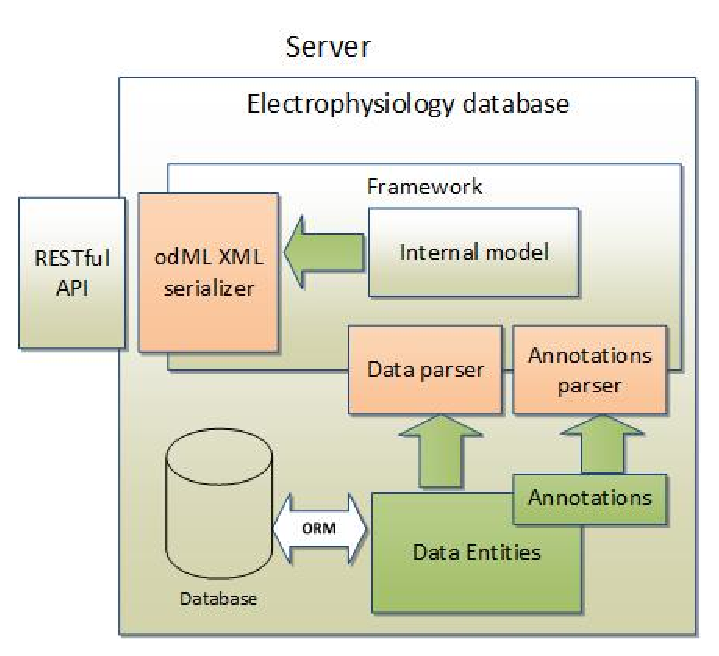
\includegraphics[width=7.5cm, height=6cm]{Framework}
\caption{\label{framework}Framework for Generating Templates and Data Transfer}
\end{figure}

\subsection{Mobile Client}

The mobile client is a framework implemented for the Android platform. A client block diagram is shown in Figure \ref{client}. A client input point is an odML deserializer that parses an input odML document into an internal model. The internal model can contain both data and templates. When the client requests a template, this template is transferred to a layout using a layout generator. When the client is requesting data for a specific layout, these data are processed by a data parser. Both layouts and data are stored in an embedded database (SQLLite). It enables users to work offline.

\begin{figure}
\centering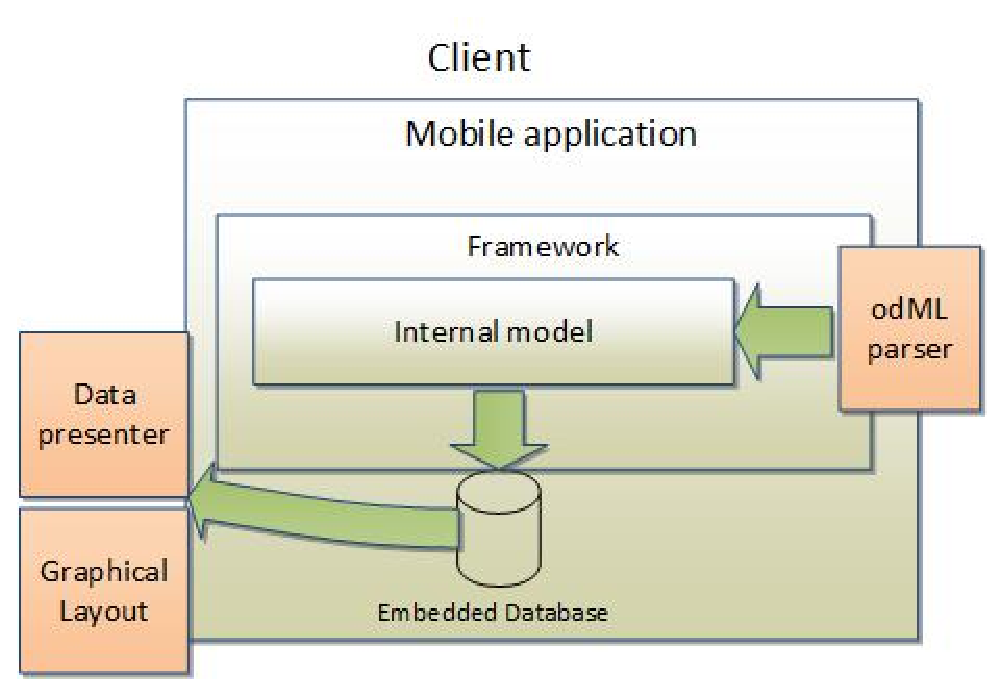
\includegraphics[width=7.5cm, height=6cm]{Client}
\caption{\label{client}Framework Implemented in the Mobile Client}
\end{figure}


\section{Use Case}

\subsection{Domain Specialization}

The main focus of the research group are methods and techniques of electroencephalography (EEG) and event-related-potentials (ERP). Experiments are conducted in a dedicated laboratory equipped with highly specialized hardware and software. Besides this laboratory, we are equipped with a mobile laboratory that enables us to perform experiments outside. In addition we are collaborating between several INCF National Nodes, including German, Belgian, Czech, USA or Japan Nodes. Our equipment and a lot of discussion with our colleagues motivate us to design and test the solution described.

Experimental procedure follows several steps.  Experiments are performed according to defined scenario. Then data and metadata are collected. These data are analyzed and results are stored and published. The central point of this infrastructure is EEGBase (XXX - ommited for review process) that serves for storing and management of EEG/ERP experiments.

Although the system uses a web-based interface, many experiments are conducted outside the laboratory where a common computer, or Internet access are not available. The aim of this use case is to validate the integration of the presented framework and generation of templates according to data structure. Generation of templates is controlled by an Android phone. When the template is generated, new data can be collected and synchronized with EEGBase.

\subsection{EEGBase} \label{Portal}



EEGBase\footnote{https://eegdatabase.kiv.zcu.cz} provides a simple wizard that guides the user when uploading experiments. The user is instructed what metadata have to be filled in. The collected metadata respecting experience of our research partners with designing and performing experiments and experimental scenarios. The metadata follow ontology described in (XXX - ommited for review process). A user interface preview is shown in Figure \ref{portal}.

The core structure contains the following semantic metadata groups:

\begin{itemize}
\item Scenario of experiment (name, length, description, ...)
\item Experimenters, tested people, experiment owner (given name, surname, contact, experiences, handicaps, ...)
\item Description of raw data (format, sampling frequency, ...)
\item Additional metadata in codebooks (weather, notes, electrode settings, artifact information, ...)
\end{itemize}


\begin{figure}
\centering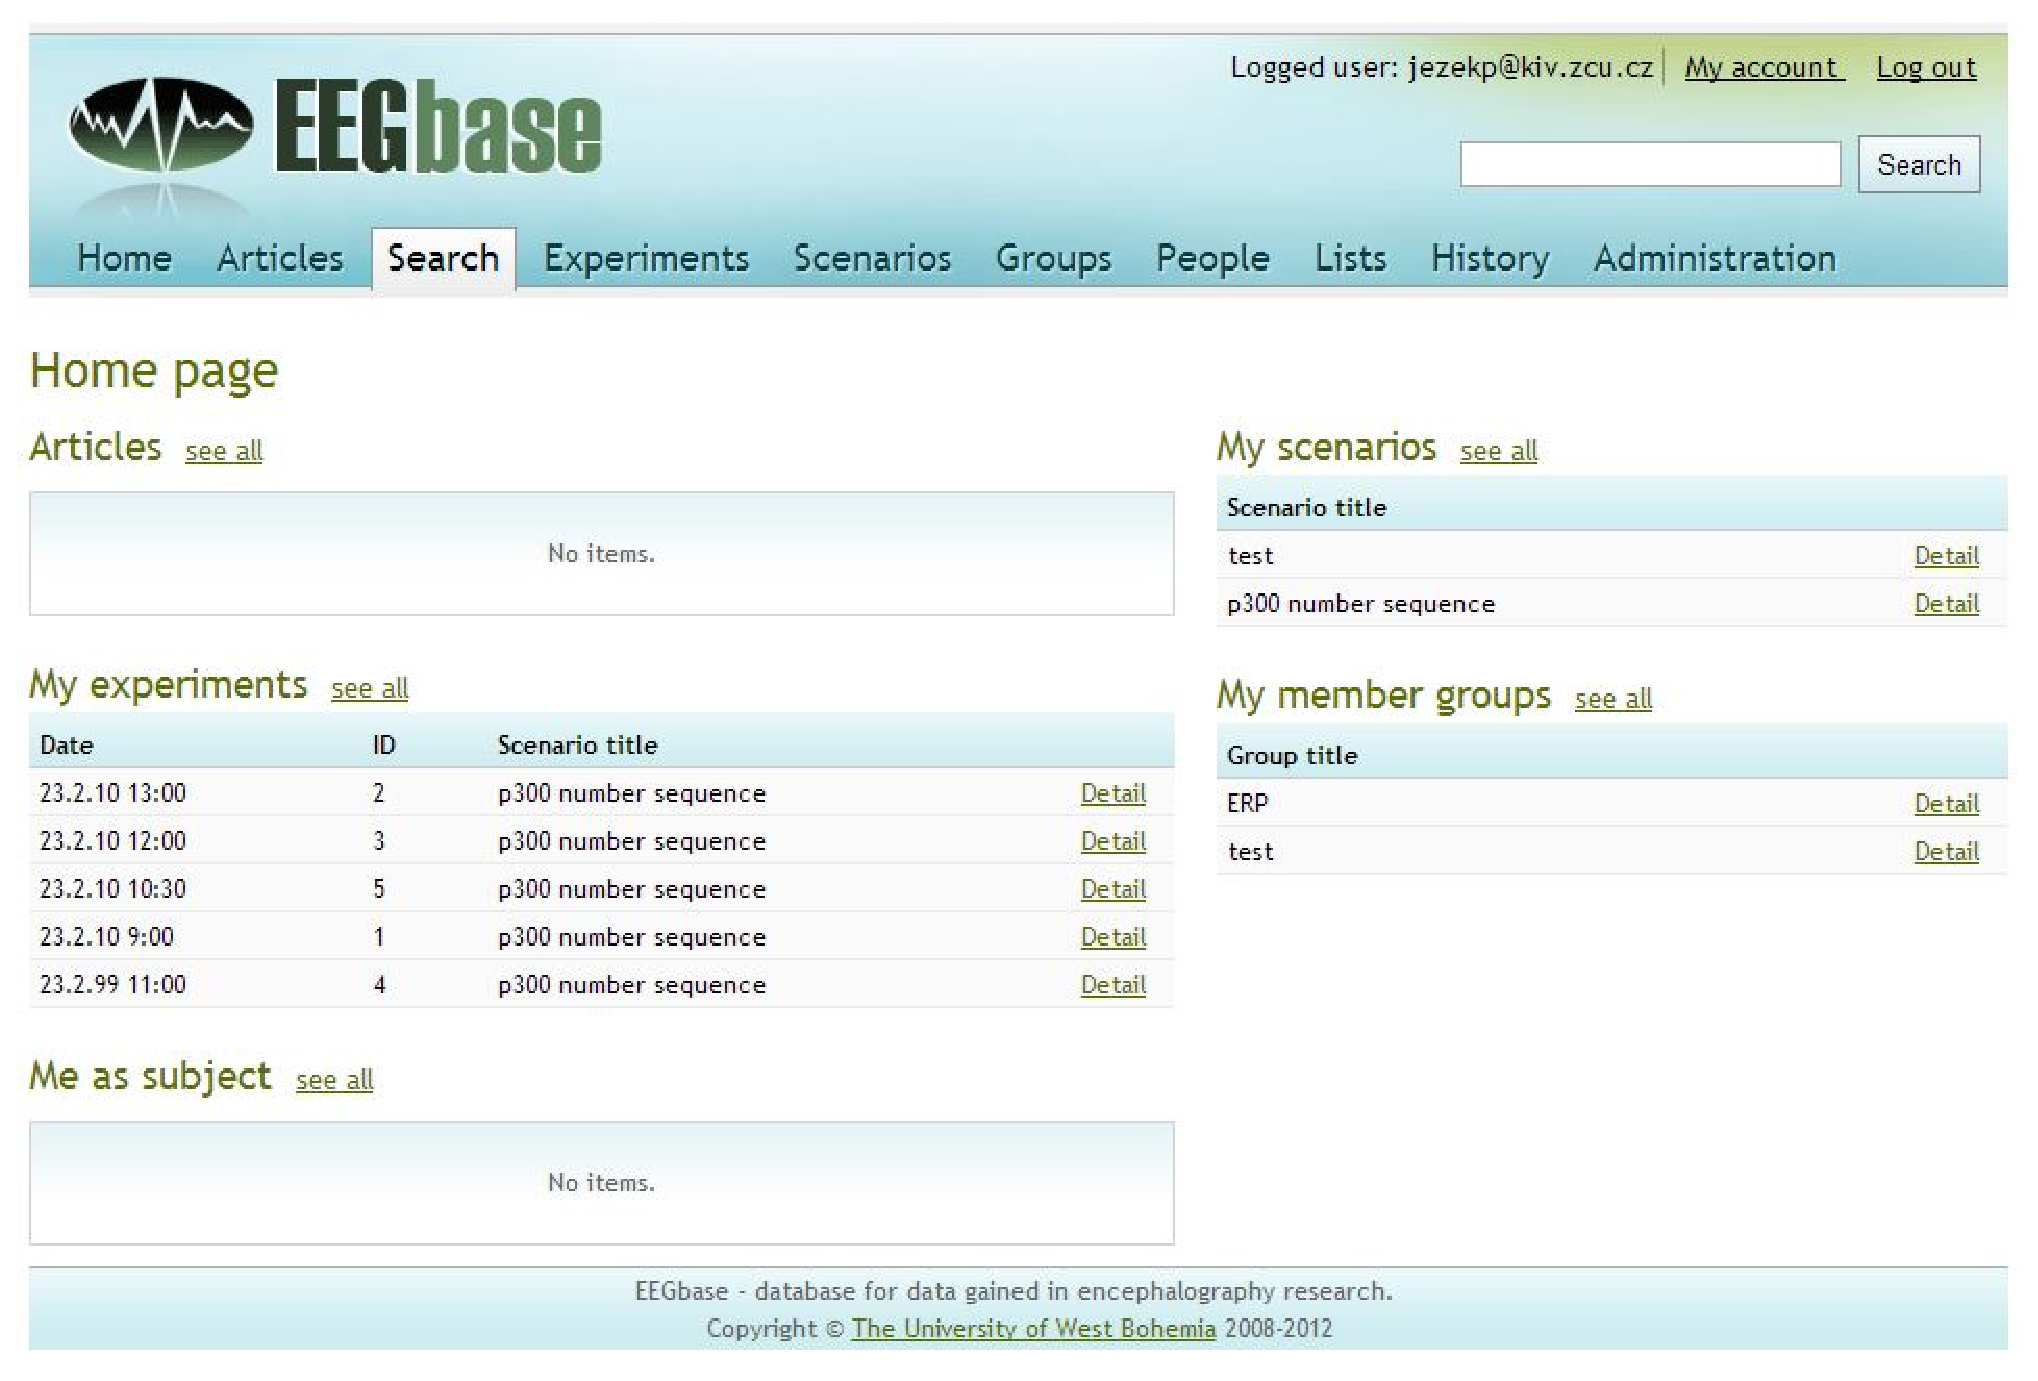
\includegraphics[width=8cm, height=5cm]{portal_preview}
\caption{\label{portal}EEGBase Preview}

\end{figure}

We prepared a simple proof-of-concept implementation based on a restricted set of metadata to demonstrate functionality of the framework. We selected the most important medata and annotate them by described annotations. Table \ref{entities_and_fields} shows selected entities with their annotated attributes.


\begin{table}
\begin{tabular}{|l|l|}
\hline
Entity & Annotated fields\\
\hline
Person     &
\begin{tabular}[c]{@{}l@{}}

@FormItem\\
	private String email;\\
	@FormItem(required = true)\\
	private String givenname;\\
	@FormItem(required = true)\\
	private String surname;\\
	@FormItem\\
	private Timestamp dateOfBirth;\\
	@FormItem(required = true)\\
	@FormItemRestriction(values = {"M", "F"})\\
	private char gender;\\
	@FormItem(required = true)\\
	@FormItemRestriction(values = {"L", "R", "X"}, defaultValue = "X")\\
	private char laterality;\\
	private String phoneNumber;\\
	@FormItem\\
	private String note;

\end{tabular} \\
\hline
Scenario   &
\begin{tabular}[c]{@{}l@{}}


	@FormItem(required = true)\\
	private Person person;\\
	@FormItem(required = true)\\
	private ResearchGroup researchGroup;\\
	@FormItem(required = true)\\
	private String title;\\
	@FormItem\\
    @FormItemRestriction(minLength =0)\\
	private int scenarioLength;\\
	@FormItem\\
	private boolean privateScenario;\\
	@FormItem\\
    @FormItemRestriction(maxLength = 255)\\
	private String description;\\
	@FormItem\\
	private String scenarioName;\\
	@FormItem\\
	private String mimetype;

\end{tabular} \\
\hline
Experiment &

\begin{tabular}[c]{@{}l@{}}

@FormItem(required = true)  \\
Weather weather;     \\
@FormItem(required = true, label = "Subject person")\\
private Person personBySubjectPersonId;\\
	@FormItem(required = true)\\
private Scenario scenario;\\
	@FormItem(required = true, label = "Owner")\\
private Person personByOwnerId;\\
	@FormItem(required = true)\\
private ResearchGroup researchGroup;\\
	@FormItem(required = true)\\
private Digitization digitization;\\
	@FormItem(required = true)\\
private SubjectGroup subjectGroup;\\
	@FormItem(required = true)\\
private Artifact artifact;\\
	@FormItem(required = true)\\
private ElectrodeConf electrodeConf;\\
	@FormItem(preview = PreviewLevel.MAJOR)\\
private Timestamp startTime;\\
	@FormItem\\
private Timestamp endTime;\\
	@FormItem\\
private int temperature;\\
	@FormItem\\
private boolean privateExperiment;\\
	@FormItem(preview = PreviewLevel.MINOR)\\
private String environmentNote;
\end{tabular}  \\

Stimulus   &
\begin{tabular}[c]{@{}l@{}}

@FormItemRestriction(maxLength = 255)\\
String description

\end{tabular} \\
\hline
DataFile   &

\begin{tabular}[c]{@{}l@{}}

@FormItemRestriction(maxLength = 255)\\
String description\\

\end{tabular}\\
\hline
\end{tabular}
\caption{Entities and their Annotated Fields}\label{entities_and_fields}
\end{table}

Since EEGBase implements RESTful web services \cite{Richardson:2007:RWS:1406352}, control of the framework API by client requests is ensured. We implemented two methods; one for listing available templates and the second one for downloading a selected template\footnote{All API methods all described more in detail in a project wiki page: https://github.com/INCF/eeg-database/wiki/RESTful-API}.



\begin{figure*}
% Use the relevant command to insert your figure file.
% For example, with the graphicx package use
\begin{tabular}{c}
\subfloat[The user can create a new workspace]{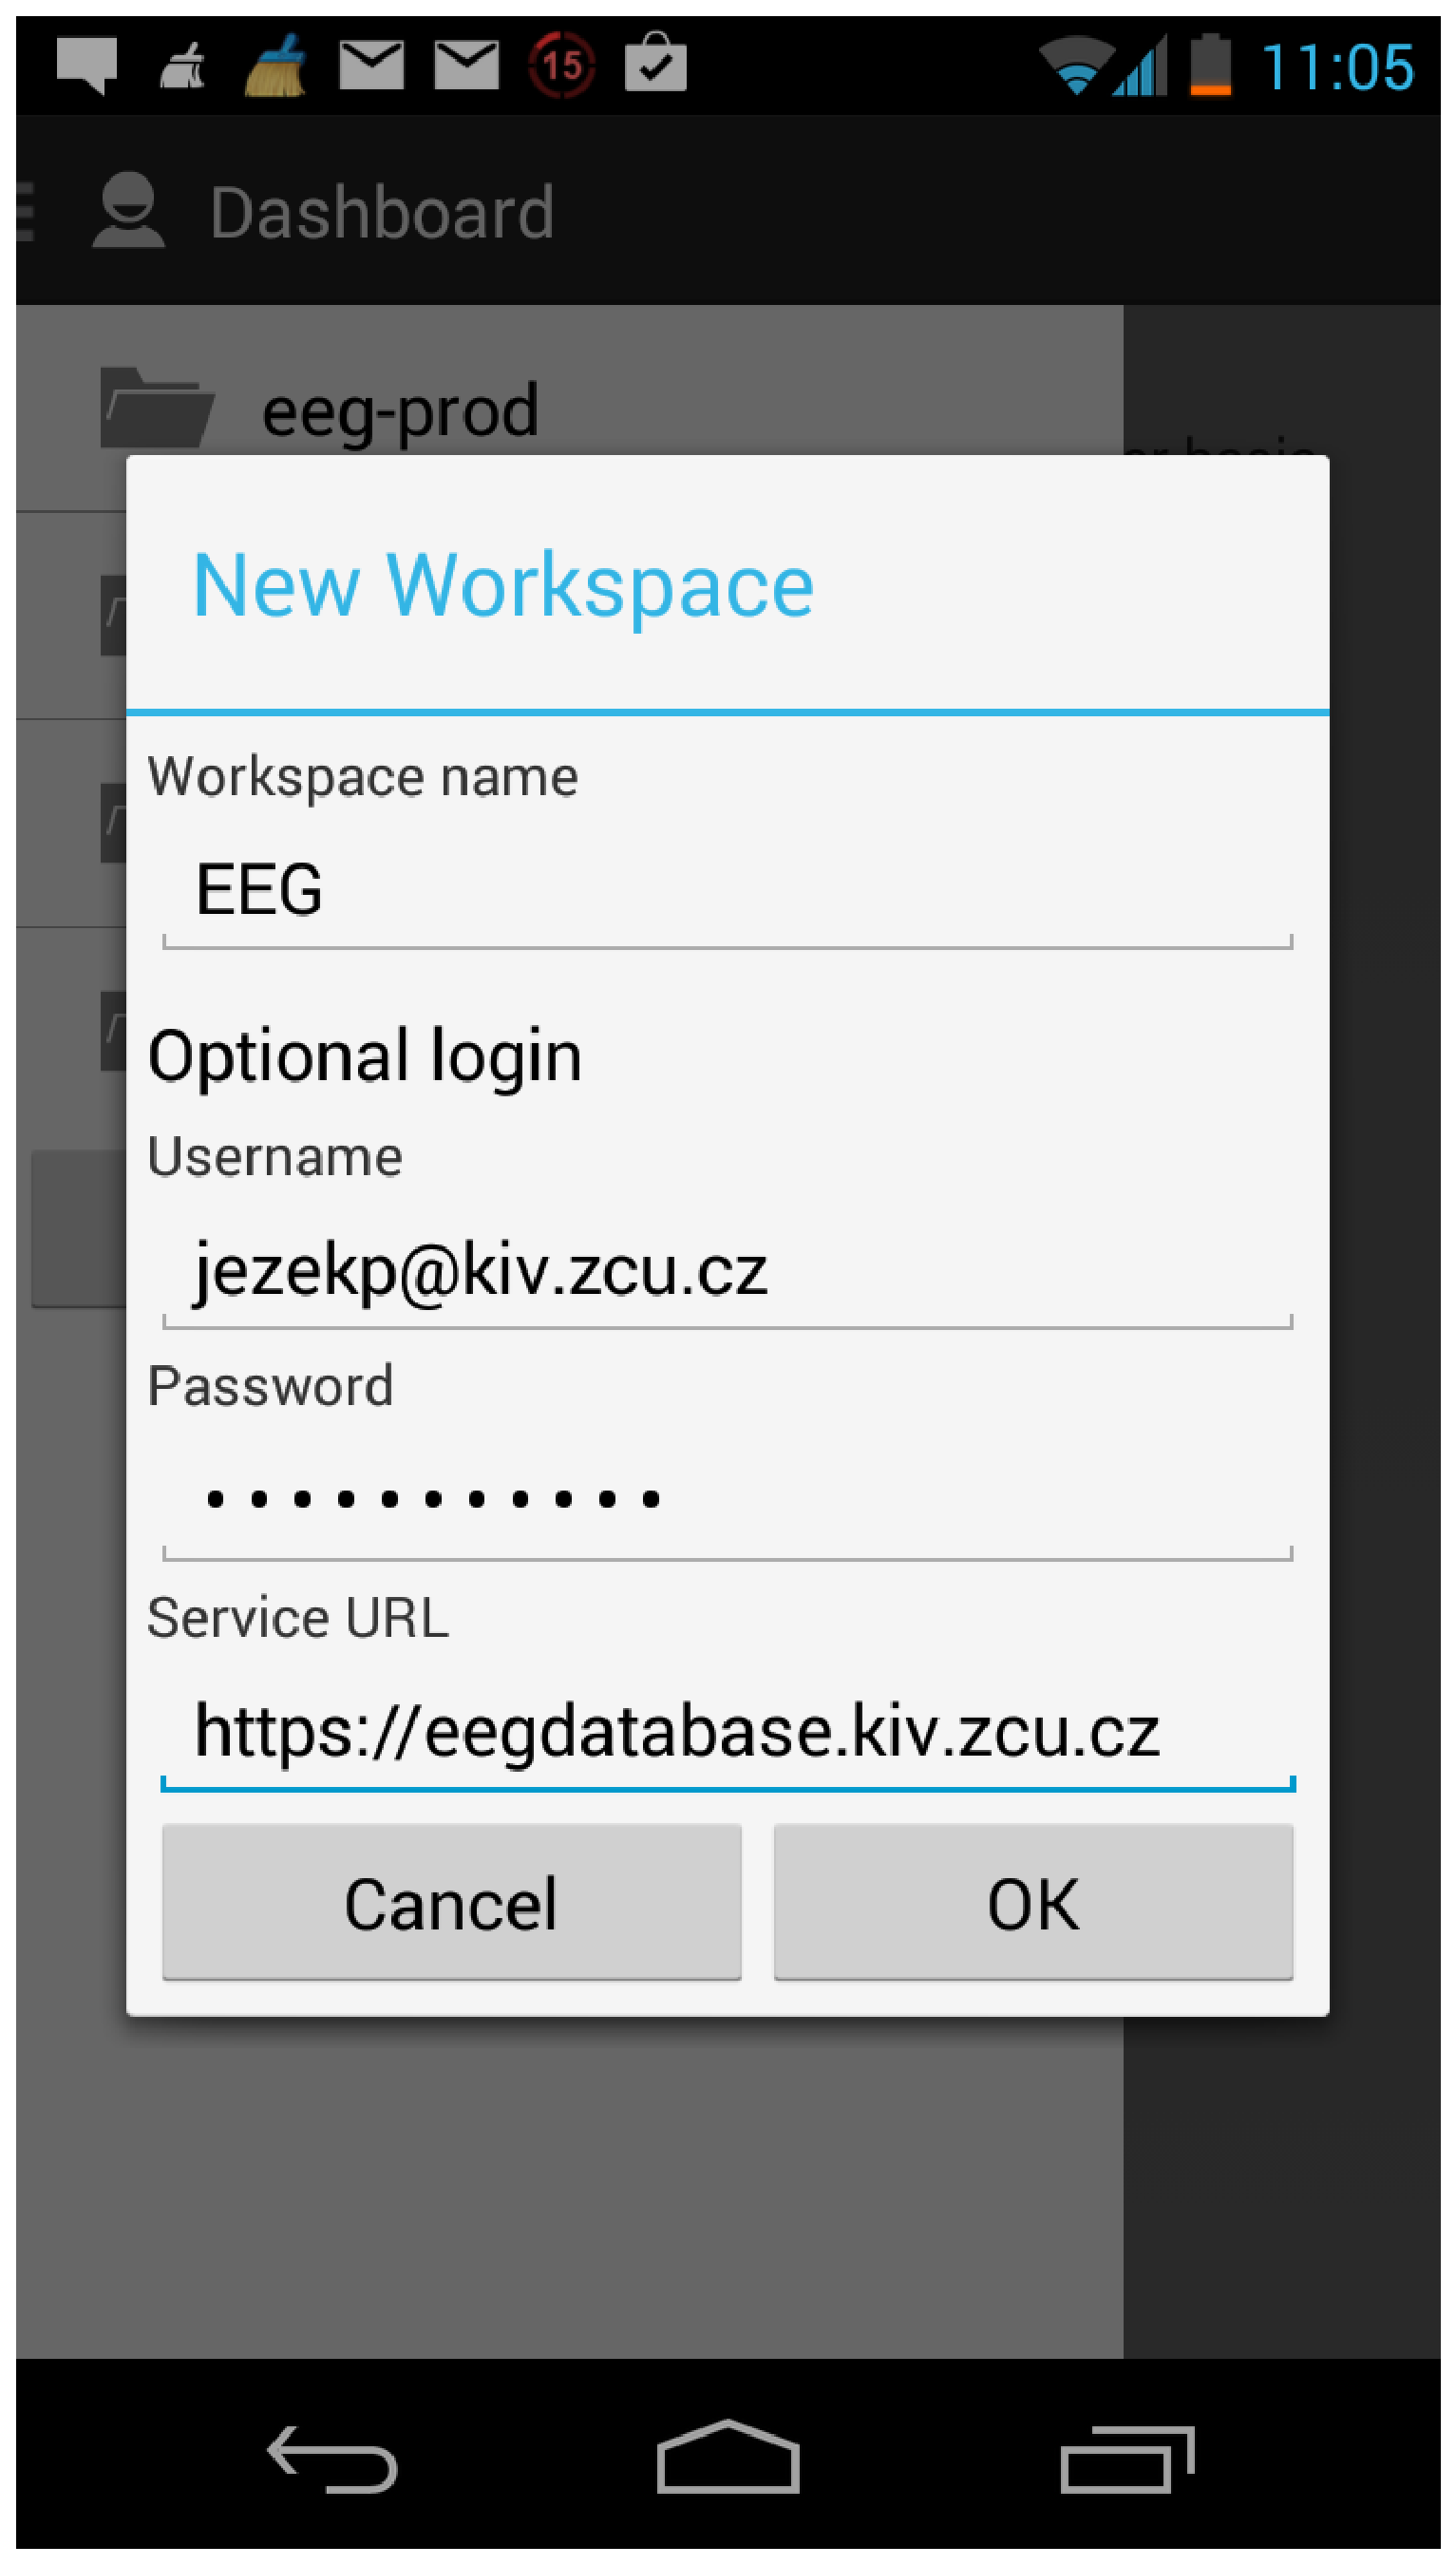
\includegraphics[width = 3.5cm, height=5.5cm]{2014-07-02090600}\label{fig:mob_app_preva}}
\hspace{10pt}\subfloat[Then select available layout]{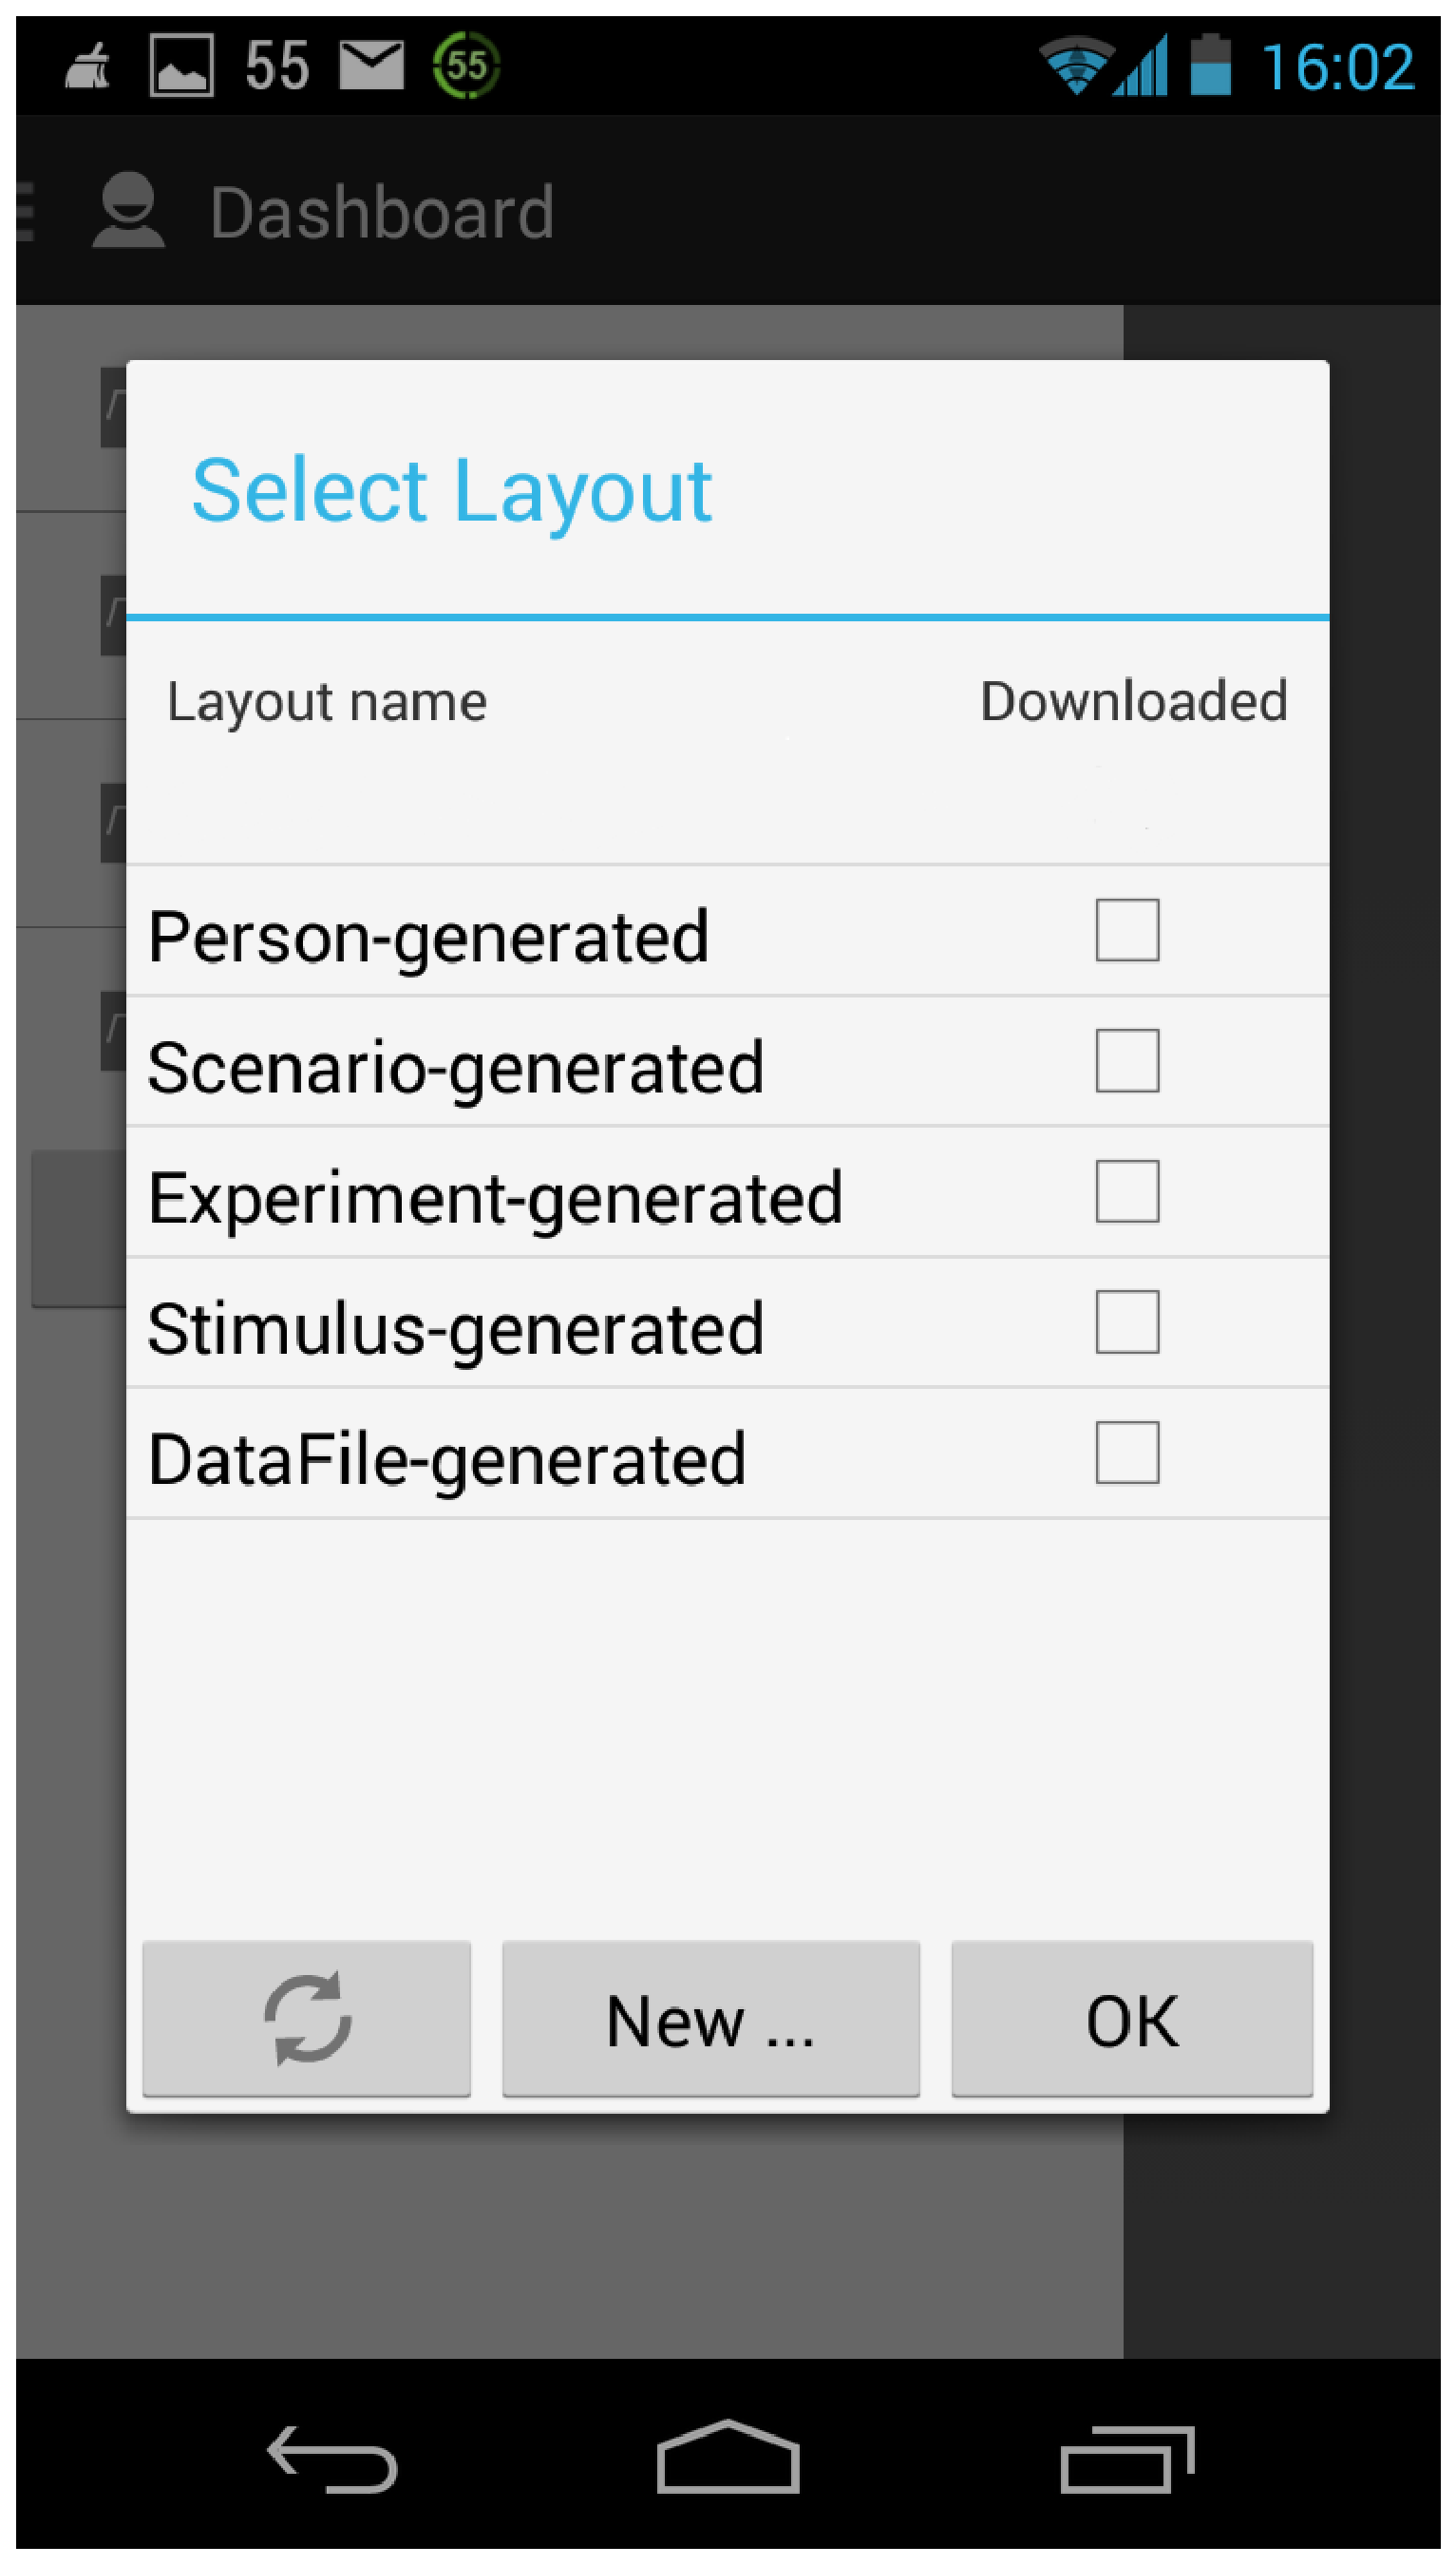
\includegraphics[width = 3.5cm, height=5.5cm]{2014-06-26140214}\label{fig:mob_app_prevb}}
\hspace{10pt}\subfloat[Finally list data]{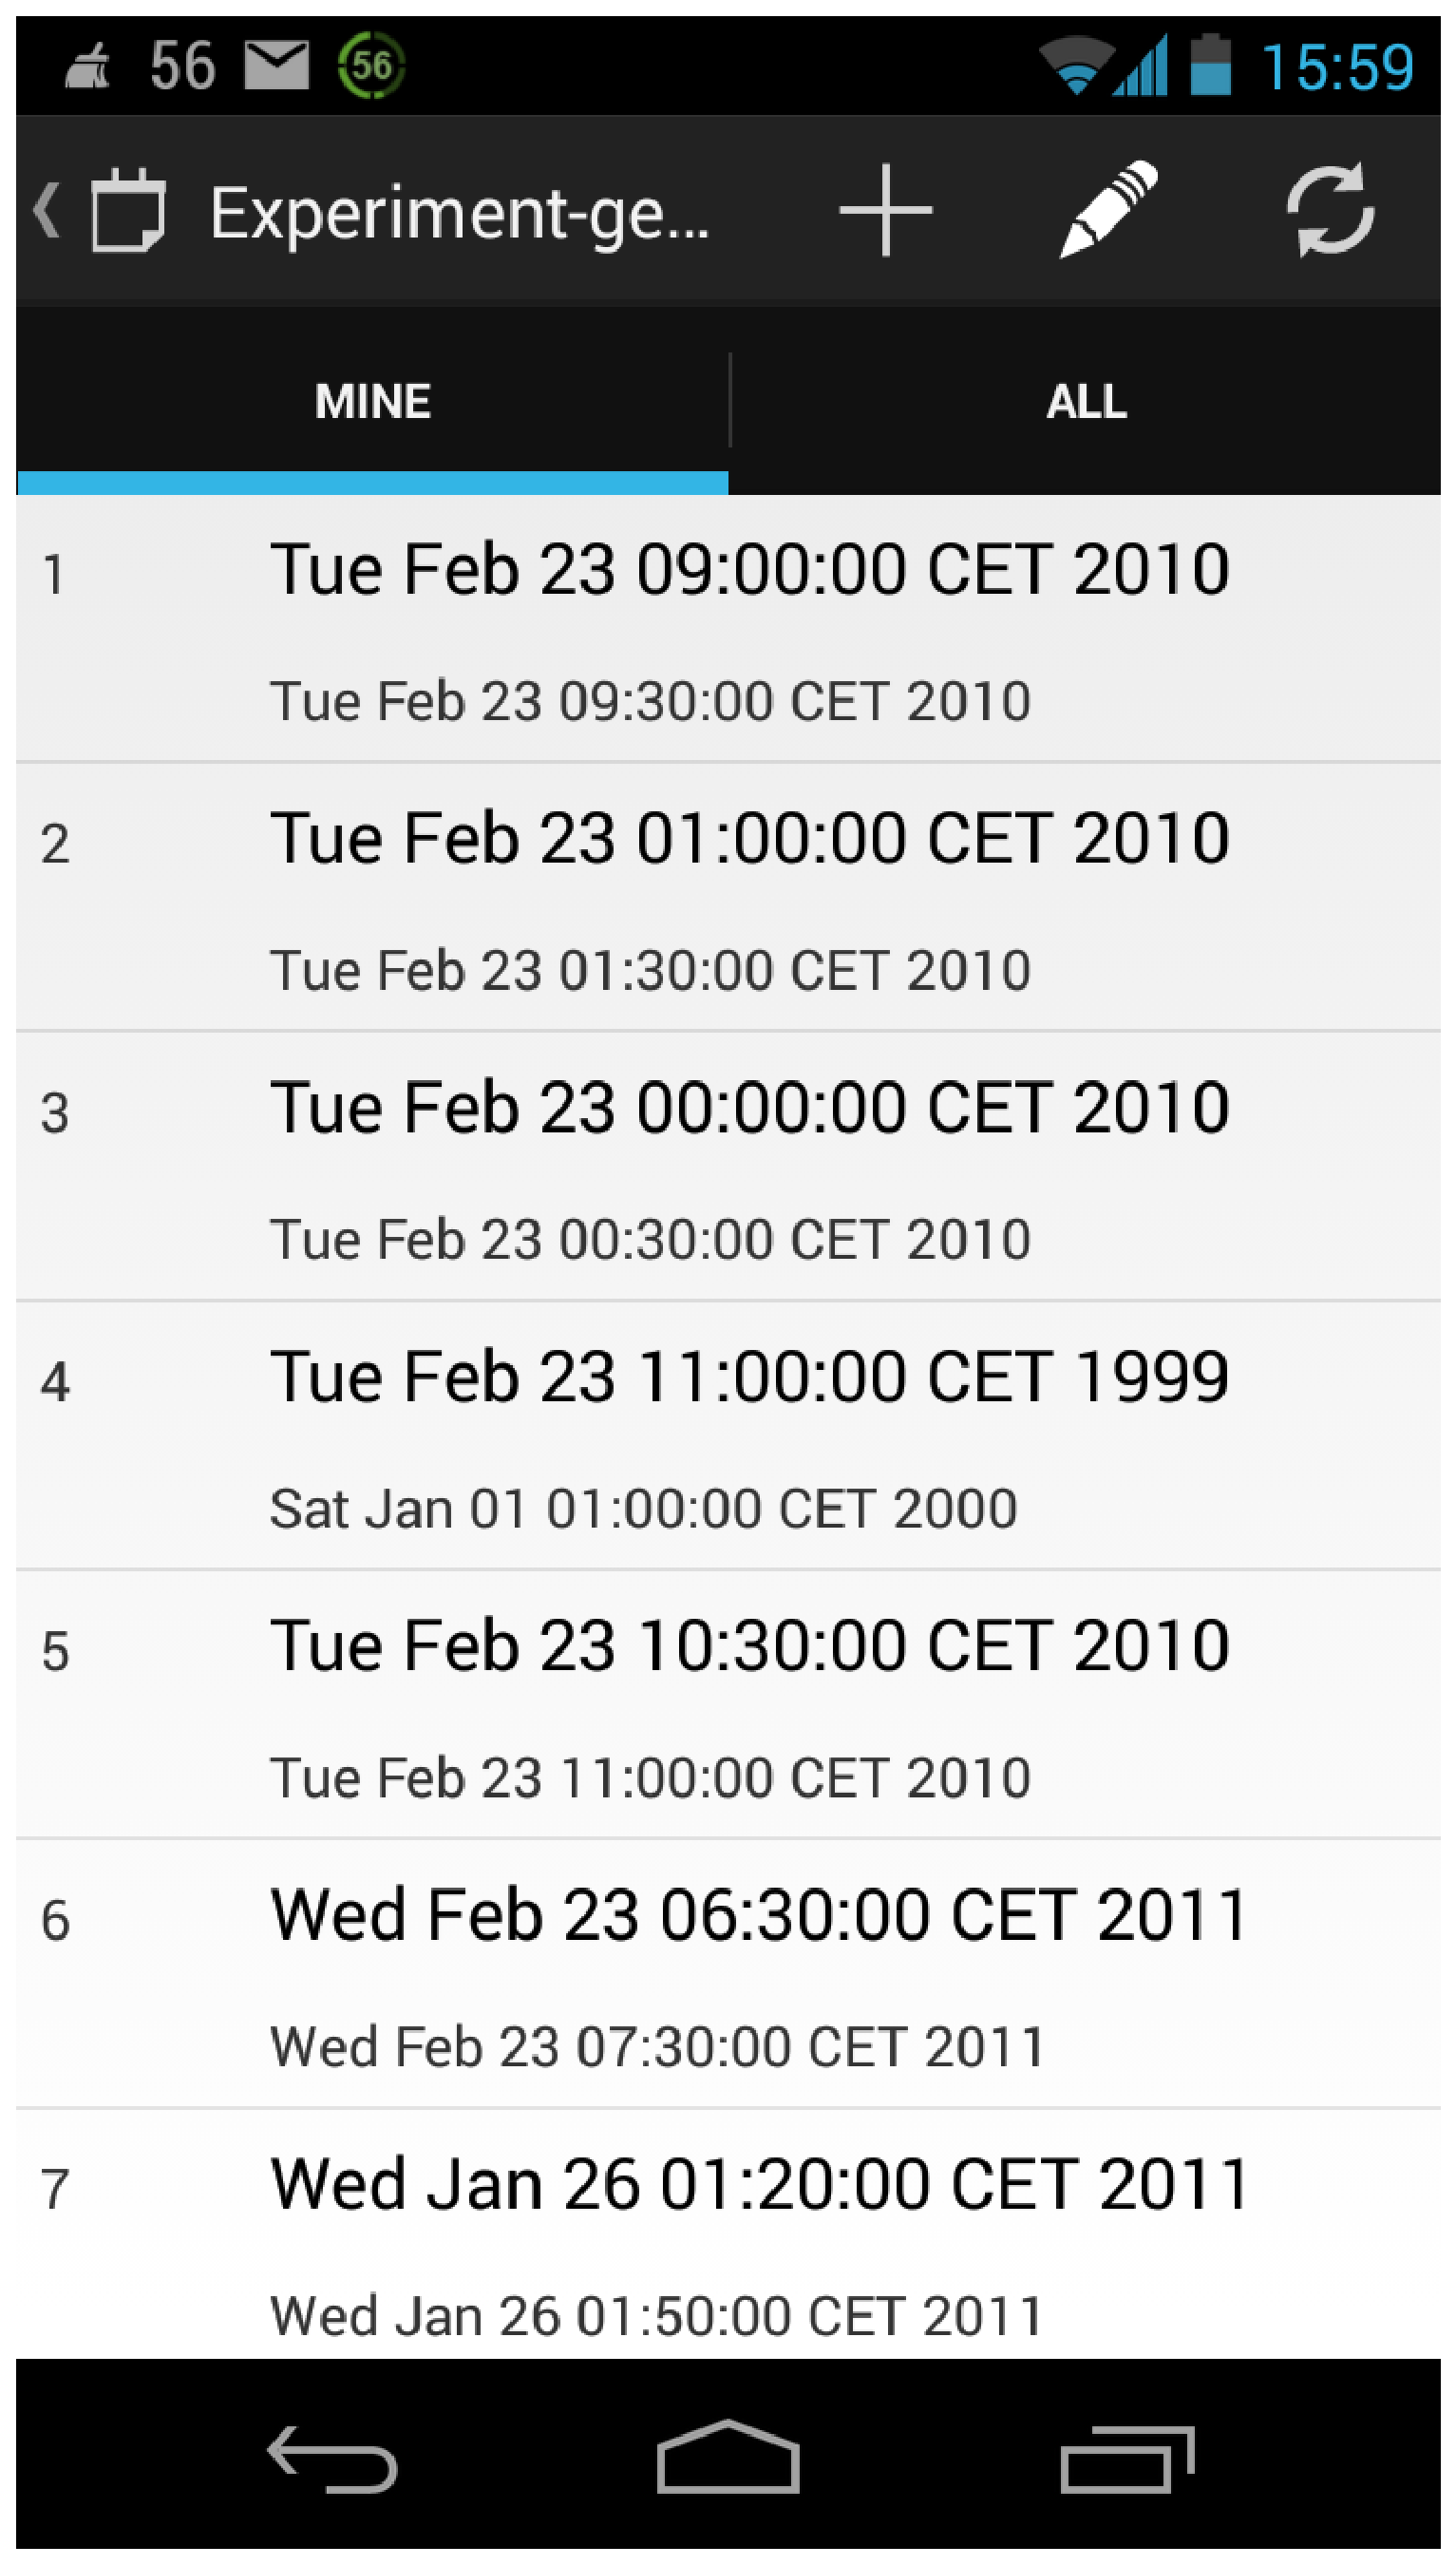
\includegraphics[width = 3.5cm, height=5.5cm]{2014-06-26135912}\label{fig:mob_app_prevc}}
\hspace{10pt}\subfloat[He/she can add a new item when clicks to a + button]{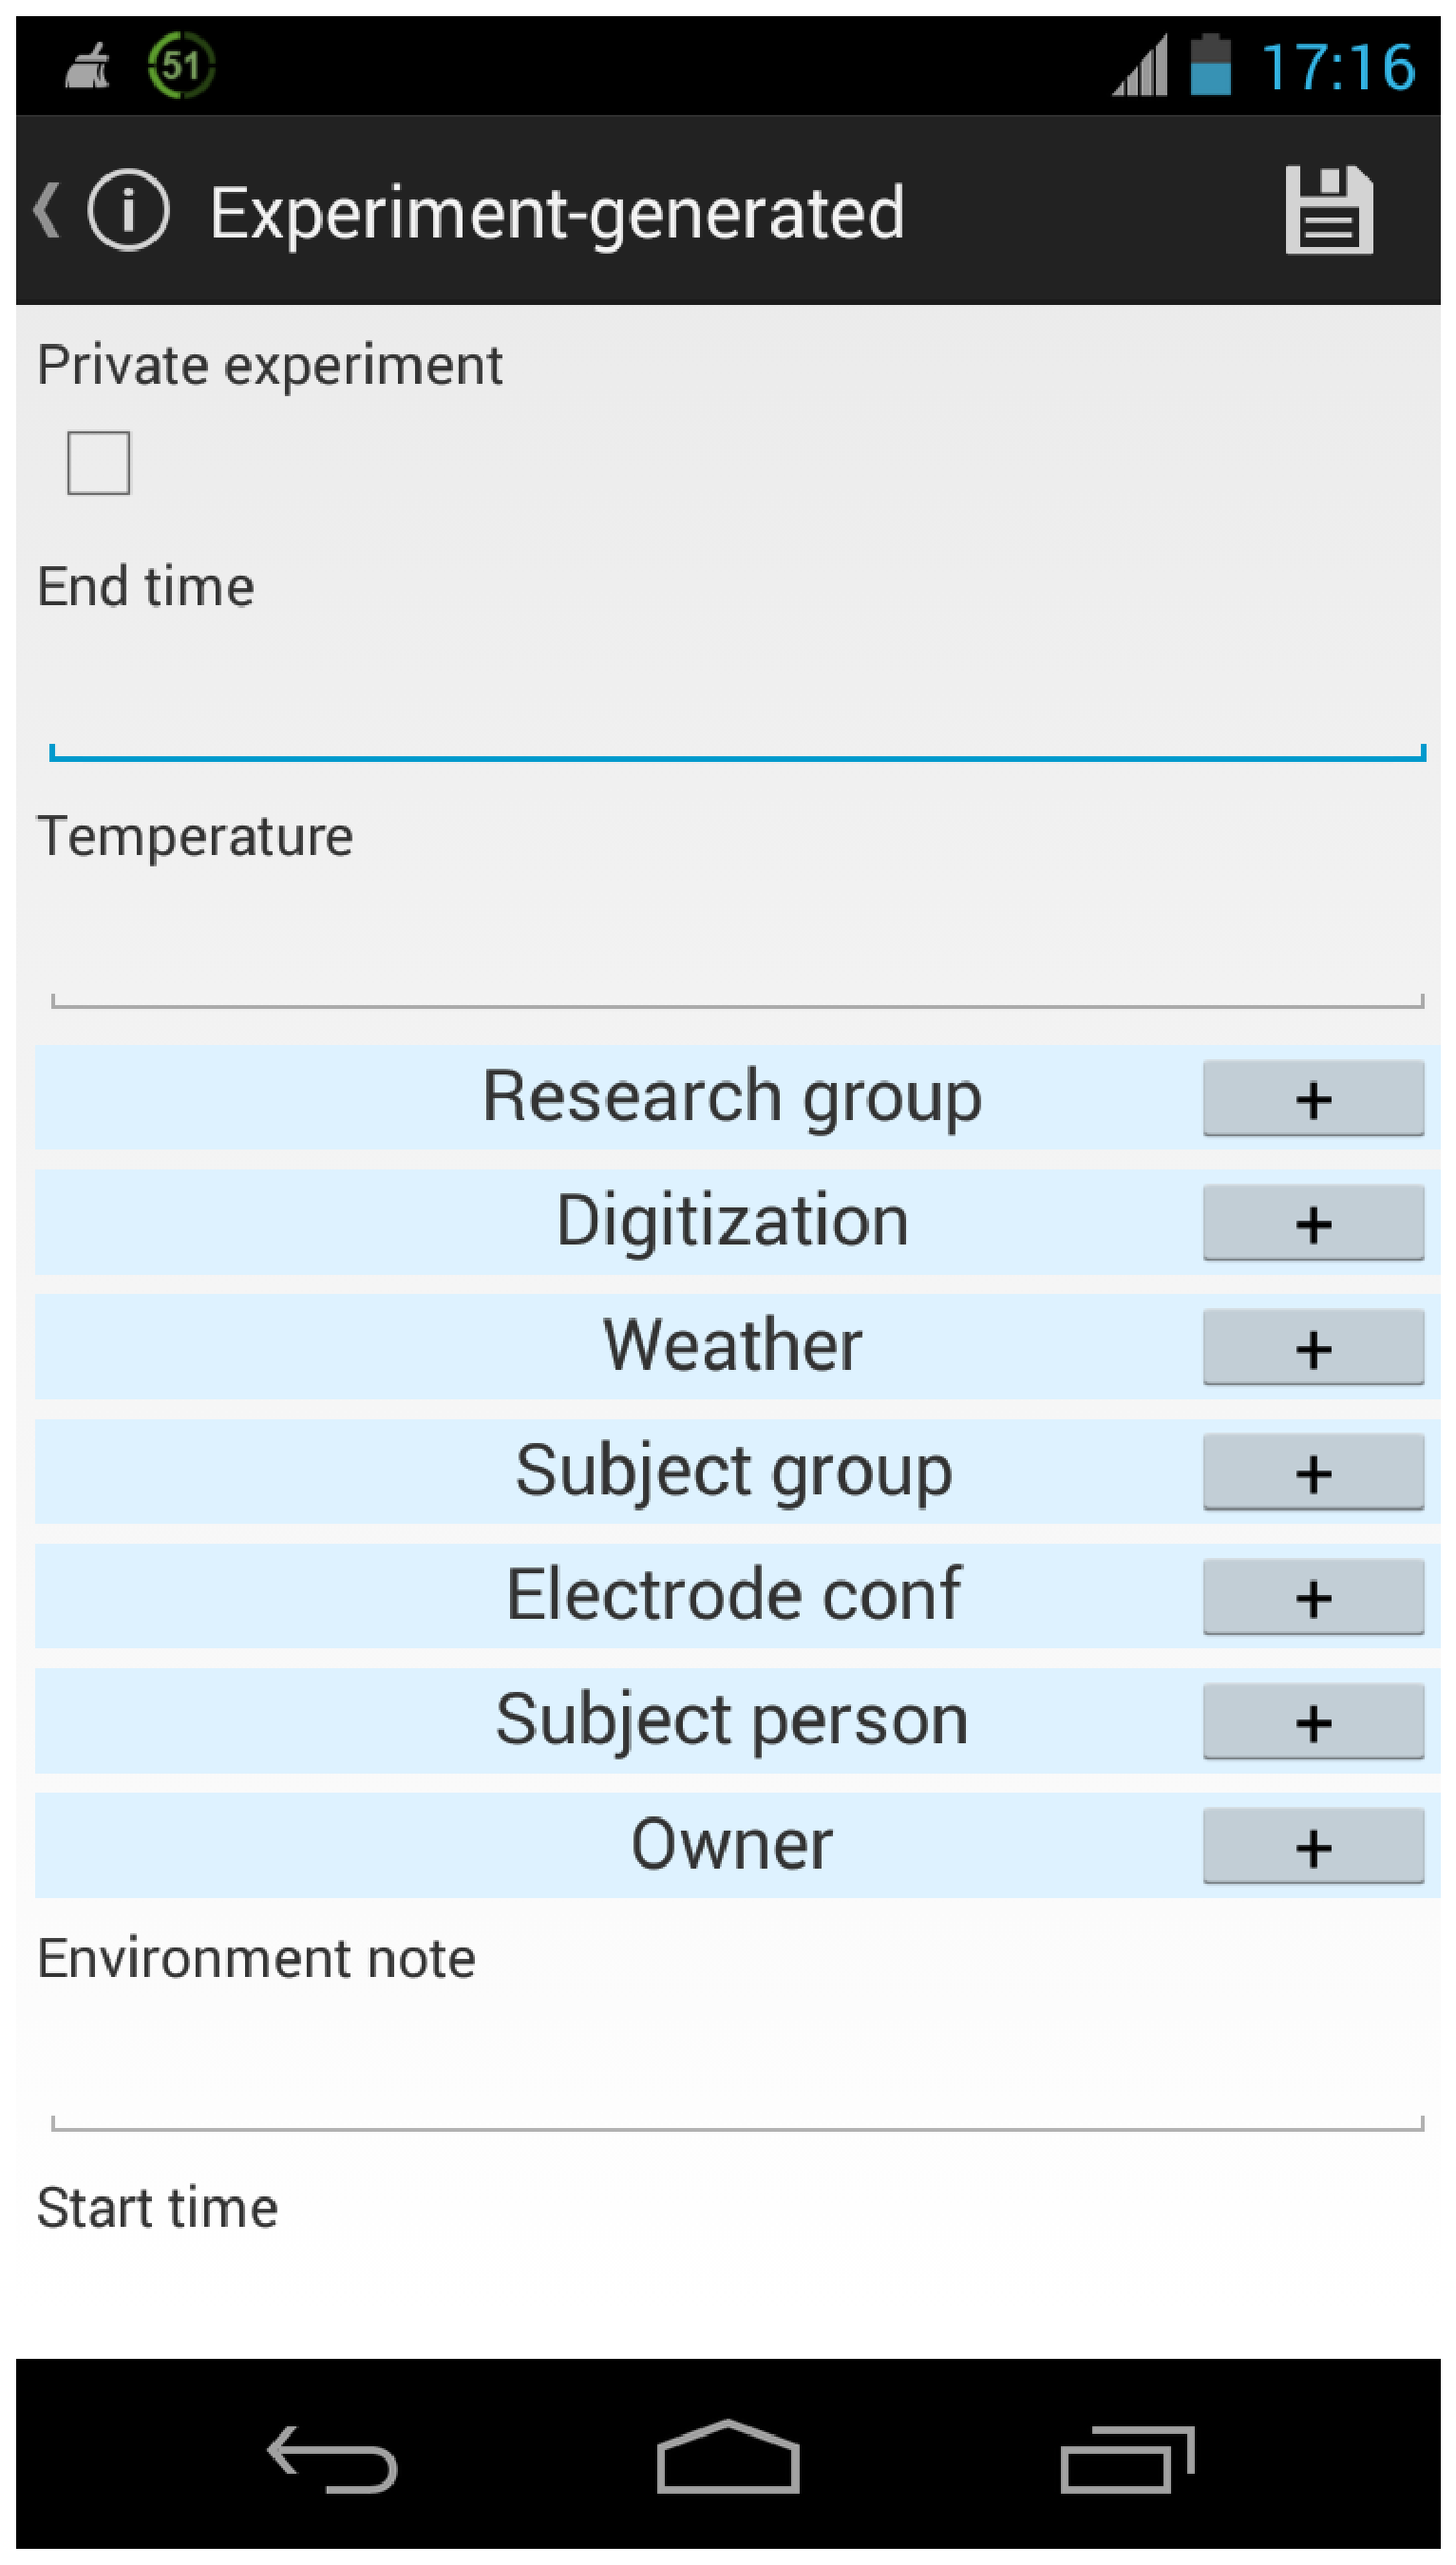
\includegraphics[width = 4cm, height=7cm]{2014-07-03151609}\label{fig:mob_app_prevd}}
\end{tabular}
% figure caption is below the figure
\caption{Mobile Application Use Case Preview}
\label{fig:mob_app_prev}
\end{figure*}

\subsection{Mobile Client} \label{Mobile_Client}

The mobile client uses common design of Android applications. Main activities of the use-case study are shown in several screen-shots in Figure \ref{fig:mob_app_prev}. Because the client is intended to work with various electrophysiological databases, it enables creating separate workspaces where each workspace works with different user credentials. In Figure \ref{fig:mob_app_preva} the user creates a new workspace. Users credentials are optional because the client can work as a stand alone system as well. In Figure \ref{fig:mob_app_prevb} available layouts are listed; the user can download them. Finally, in Figure \ref{fig:mob_app_prevc} the user can download data from the server or add new data as shown in Figure \ref{fig:mob_app_prevd}.

By following the described steps we created one workspace connected to EEGBase (see Figure\ref{fig:mob_app_preva}) and downloaded available layouts (Person, Scenario, Experiment and DataFile as listed in Figure \ref{fig:mob_app_prevb}). When the layouts were downloaded experiments from the server were listed (see Figure \ref{fig:mob_app_prevc}). Finally, we add several new experiments using form listed in Figure \ref{fig:mob_app_prevd}. These experiments were stored on the server.



% An example of a floating figure using the graphicx package.
% Note that \label must occur AFTER (or within) \caption.
% For figures, \caption should occur after the \includegraphics.
% Note that IEEEtran v1.7 and later has special internal code that
% is designed to preserve the operation of \label within \caption
% even when the captionsoff option is in effect. However, because
% of issues like this, it may be the safest practice to put all your
% \label just after \caption rather than within \caption{}.
%
% Reminder: the "draftcls" or "draftclsnofoot", not "draft", class
% option should be used if it is desired that the figures are to be
% displayed while in draft mode.
%
%\begin{figure}[!t]
%\centering
%\includegraphics[width=2.5in]{myfigure}
% where an .eps filename suffix will be assumed under latex,
% and a .pdf suffix will be assumed for pdflatex; or what has been declared
% via \DeclareGraphicsExtensions.
%\caption{Simulation Results}
%\label{fig_sim}
%\end{figure}

% Note that IEEE typically puts floats only at the top, even when this
% results in a large percentage of a column being occupied by floats.


% An example of a double column floating figure using two subfigures.
% (The subfig.sty package must be loaded for this to work.)
% The subfigure \label commands are set within each subfloat command, the
% \label for the overall figure must come after \caption.
% \hfil must be used as a separator to get equal spacing.
% The subfigure.sty package works much the same way, except \subfigure is
% used instead of \subfloat.
%
%\begin{figure*}[!t]
%\centerline{\subfloat[Case I]\includegraphics[width=2.5in]{subfigcase1}%
%\label{fig_first_case}}
%\hfil
%\subfloat[Case II]{\includegraphics[width=2.5in]{subfigcase2}%
%\label{fig_second_case}}}
%\caption{Simulation results}
%\label{fig_sim}
%\end{figure*}
%
% Note that often IEEE papers with subfigures do not employ subfigure
% captions (using the optional argument to \subfloat), but instead will
% reference/describe all of them (a), (b), etc., within the main caption.


% An example of a floating table. Note that, for IEEE style tables, the
% \caption command should come BEFORE the table. Table text will default to
% \footnotesize as IEEE normally uses this smaller font for tables.
% The \label must come after \caption as always.
%
%\begin{table}[!t]
%% increase table row spacing, adjust to taste
%\renewcommand{\arraystretch}{1.3}
% if using array.sty, it might be a good idea to tweak the value of
% \extrarowheight as needed to properly center the text within the cells
%\caption{An Example of a Table}
%\label{table_example}
%\centering
%% Some packages, such as MDW tools, offer better commands for making tables
%% than the plain LaTeX2e tabular which is used here.
%\begin{tabular}{|c||c|}
%\hline
%One & Two\\
%\hline
%Three & Four\\
%\hline
%\end{tabular}
%\end{table}


% Note that IEEE does not put floats in the very first column - or typically
% anywhere on the first page for that matter. Also, in-text middle ("here")
% positioning is not used. Most IEEE journals/conferences use top floats
% exclusively. Note that, LaTeX2e, unlike IEEE journals/conferences, places
% footnotes above bottom floats. This can be corrected via the \fnbelowfloat
% command of the stfloats package.

\section{Future Work}

The proposed solution works satisfactorily and the presented use-case study validates its functionality on real data. However, the presented pilot implementation has several gaps that are planned to be overcome.

First, we will focus our effort on developing the mobile client to offer the possibility to create templates natively on the client, allowing to work offline. For this purpose, we will merge efforts between the EEGBase client and the mobile odML editor (XXX - ommited for review process) to propose a unique mobile client that would work on both database. With this work, we will be able to extend 1- the interoperability between these two resources and 2- extend the functionalities of the mobile client presented here to iOS and ultimately to more platforms\footnote{several frameworks as http://phonegap.com/ enables development of platform independent mobile applications}.
Secondly, we will address the problem of data and metadata storage on both client and server sides. As electrophysiological data are heterogeneous, the usage of NoSQL databases seems to be more practical. Our first tests prove (XXX - ommited for review process) that a shift from a relational database to a NoSQL one brings a lot of benefits handling metadata. The major step is to propose a suitable mapping of heterogeneous metadata stored in a NoSQL database to a suitable data template. Finally, we are planning to extend the server part of the framework to work with a larger diversity of servers than Java-based servers.



\section{Conclusion}




Experiments in electrophysiology domain produce a lot of collections of semi-structured data and metadata. To organize these metadata, various data formats implemented in electrophysiological databases have been introduced. Data in these databases are accessed from laboratory computers using fixed user interfaces. Therefore these databases are unreachable where a common computer is not available. With expansion of mobile devices users would like to manage data using their smart phones. Because the dual development of user interfaces for both common computers and mobile devices increases demands to developers and reduces users experience with these systems, we proposed an annotation framework that enables to generate graphical layouts for mobile devices automatically. This framework enables users to map a data layer of an electrophysiological database and create the template representing the data structure. This template is serialized to an odML document and transferred to the client system. The client system parses this template and generates a graphical layout displayed in the device. In addition, when the layout is prepared, the experimental data can be synchronized with the server.


% conference papers do not normally have an appendix


% use section* for acknowledgement
\section*{Acknowledgment}
(XXX - ommited for review process)

% trigger a \newpage just before the given reference
% number - used to balance the columns on the last page
% adjust value as needed - may need to be readjusted if
% the document is modified later
%\IEEEtriggeratref{8}
% The "triggered" command can be changed if desired:
%\IEEEtriggercmd{\enlargethispage{-5in}}

% references section_

% can use a bibliography generated by BibTeX as a .bbl file
% BibTeX documentation can be easily obtained at:
% http://www.ctan.org/tex-archive/biblio/bibtex/contrib/doc/
% The IEEEtran BibTeX style support page is at:
% http://www.michaelshell.org/tex/ieeetran/bibtex/
\bibliographystyle{apalike}
% argument is your BibTeX string definitions and bibliography database(s)
\bibliography{bibliography,neuroportals,frontiers}
%
% <OR> manually copy in the resultant .bbl file
% set second argument of \begin to the number of references
% (used to reserve space for the reference number labels box)


\end{document}

